\documentclass[]{article}

%These tell TeX which packages to use.
\usepackage{array,epsfig}
\usepackage{amsmath}
\usepackage{amsfonts}
\usepackage{amssymb}
\usepackage{amsxtra}
\usepackage{amsthm}
\usepackage{mathrsfs}
\usepackage{color}

%Here I define some theorem styles and shortcut commands for symbols I use often
\theoremstyle{definition}
\newtheorem{defn}{Definition}
\newtheorem{thm}{Theorem}
\newtheorem{cor}{Corollary}
\newtheorem*{rmk}{Remark}
\newtheorem{lem}{Lemma}
\newtheorem*{joke}{Joke}
\newtheorem{ex}{Example}
\newtheorem*{soln}{Solution}
\newtheorem{prop}{Proposition}

\newcommand{\lra}{\longrightarrow}
\newcommand{\ra}{\rightarrow}
\newcommand{\surj}{\twoheadrightarrow}
\newcommand{\graph}{\mathrm{graph}}
\newcommand{\bb}[1]{\mathbb{#1}}
\newcommand{\Z}{\bb{Z}}
\newcommand{\Q}{\bb{Q}}
\newcommand{\R}{\bb{R}}
\newcommand{\C}{\bb{C}}
\newcommand{\N}{\bb{N}}
\newcommand{\M}{\mathbf{M}}
\newcommand{\m}{\mathbf{m}}
\newcommand{\MM}{\mathscr{M}}
\newcommand{\HH}{\mathscr{H}}
\newcommand{\Om}{\Omega}
\newcommand{\Ho}{\in\HH(\Om)}
\newcommand{\bd}{\partial}
\newcommand{\del}{\partial}
\newcommand{\bardel}{\overline\partial}
\newcommand{\textdf}[1]{\textbf{\textsf{#1}}\index{#1}}
\newcommand{\img}{\mathrm{img}}
\newcommand{\ip}[2]{\left\langle{#1},{#2}\right\rangle}
\newcommand{\inter}[1]{\mathrm{int}{#1}}
\newcommand{\exter}[1]{\mathrm{ext}{#1}}
\newcommand{\cl}[1]{\mathrm{cl}{#1}}
\newcommand{\ds}{\displaystyle}
\newcommand{\vol}{\mathrm{vol}}
\newcommand{\cnt}{\mathrm{ct}}
\newcommand{\osc}{\mathrm{osc}}
\newcommand{\LL}{\mathbf{L}}
\newcommand{\UU}{\mathbf{U}}
\newcommand{\support}{\mathrm{support}}
\newcommand{\AND}{\;\wedge\;}
\newcommand{\OR}{\;\vee\;}
\newcommand{\Oset}{\varnothing}
\newcommand{\st}{\ni}
\newcommand{\wh}{\widehat}

%Pagination stuff.
\setlength{\topmargin}{-.3 in}
\setlength{\oddsidemargin}{0in}
\setlength{\evensidemargin}{0in}
\setlength{\textheight}{9.in}
\setlength{\textwidth}{6.5in}
\pagestyle{empty}



\begin{document}


\begin{center}
{\textbf{Experimental modeling of pyroclastic density currents}}\\
Paul A. Jarvis\\ %You should put your name here
\end{center}

\vspace{0.2 cm}

\section{Introduction and lab rules}
\label{sec:lab_rules}

In this practical, you are going to perform a set of experiments designed to model pyroclastic density currents (PDCs). These experiments will be performed in the Geophysical Fluid Dynamics laboratory of the Physical Volcanology and Geological Risk research group in the Department of Earth Sciences at the University of Geneva. This is a working laboratory and as such there are a number of piece of equipment and different experimental setups in the lab which are currently in use. \textbf{Please do not touch anything unless you are explicitly told that you can.} Additionally there are a number of laboratory rules that must be followed at all times:

\begin{enumerate}
\item Wear shoes that completely cover your feet. Wearing sandles is prohibited at all times.
\item It is forbidden to prepare, eat, drink or store any food in the laboratory.
\item In case of any accidents, burns, cuts etc., immediately notify the laboratory manager.
\item Any broken glass must be placed in the bin for glass waste.
\item Always clear up spills (liquid or particulate) immediately.
\item If people do not respect the health and safety rules, they will have to leave the practical and get no mark.
\end{enumerate}

\section{Experimental description}
\label{sec:exp}

You will be performing experiments in the large flume (Figure~\ref{fig:flume}). The flume is split into three sections. There is a leftmost gated section which we will not be using in this practical, and will be separated from the rest of the tank by a gate. Next to this is another gated section which will contain the gate fluid, whilst the rest of the tank will contain the environmental fluid. Between the environmental and gate fluids will be a gate which is removed to initiate the experiment. 

  \begin{figure}
    $$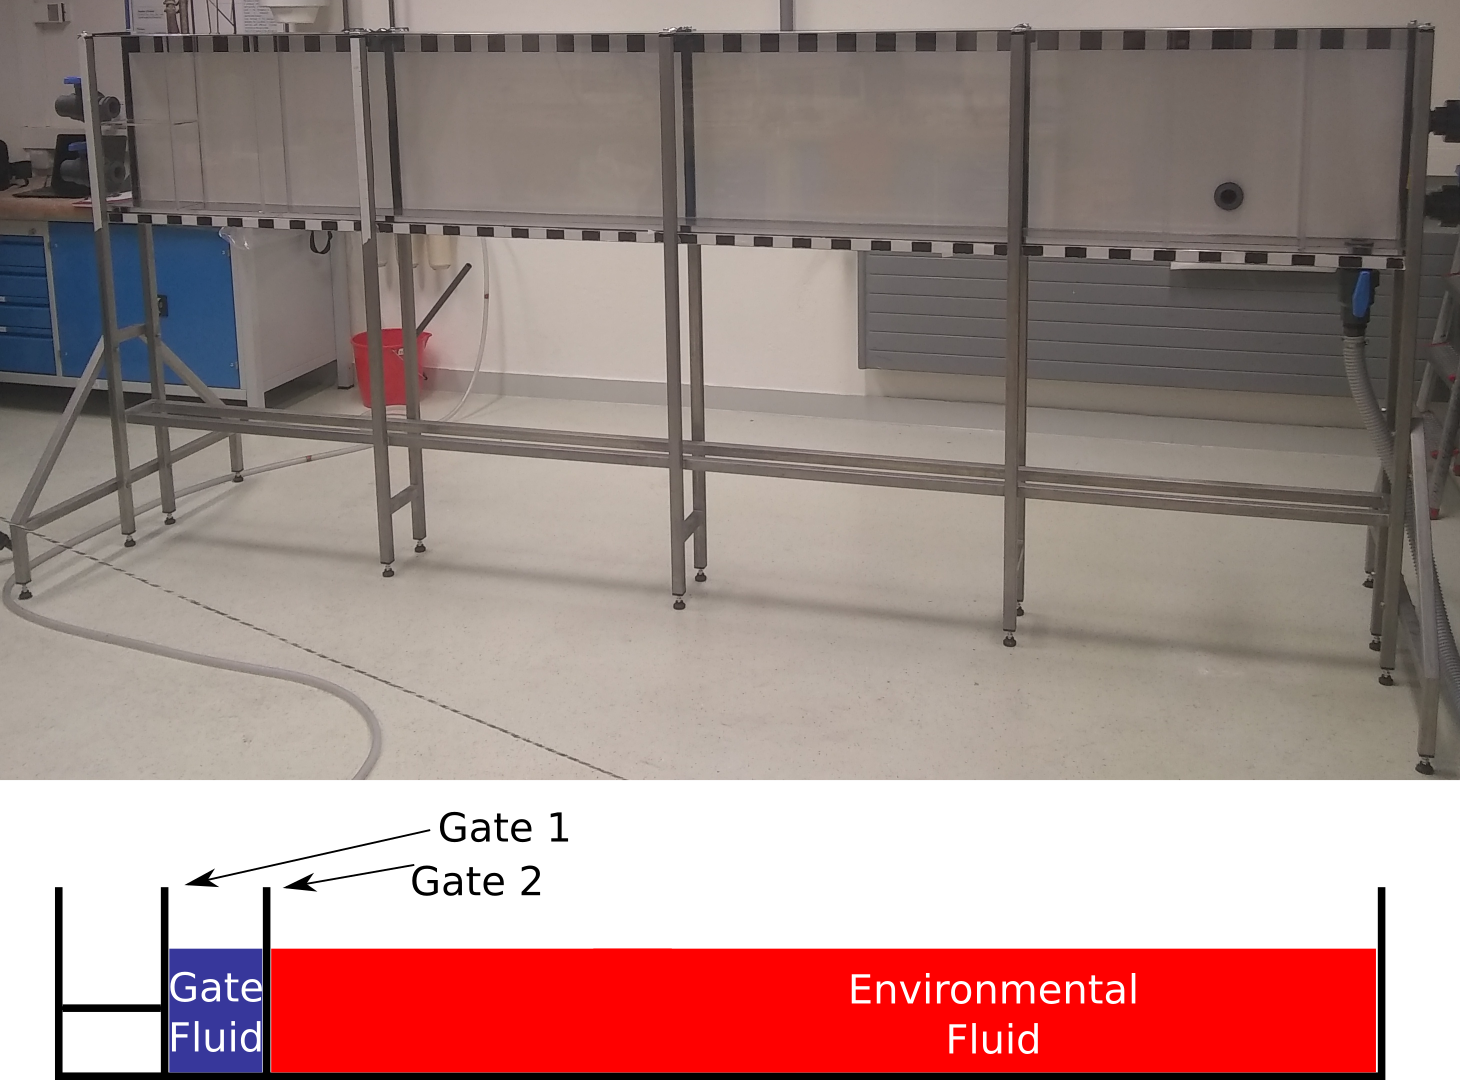
\includegraphics[width=0.75\textwidth]{flume_setup.png}$$
    \caption{The large flume in the Geophysical Fluid Dynamics laboratory. \label{fig:flume}}
  \end{figure}

  In each experiment, you will add sugar to the gate fluid to increase its density with respect to the environmental fluid. Once the gate is removed, the gate fluid will spread as a dense gravity current along the base of the tank. The objective of each experiment is to measure the position of the front of current as a function of time and determine the front velocity of the current. By performing multiple experiments, you will work out how the front velocity depends on the density difference between the two fluids.

\section{Test experiment: procedure}
\label{sec:proc}

Before performing the official experiments, we are going to perform a test experiment to help us finalise the experimental procedure and, in particular, develop our methods of data collection.

\begin{enumerate}
\item Ensure that the tank is empty and all gates are removed.
\item Use the hose to fill up the tank to a height of approximately 40 cm. \textbf{Be careful not to make a mess}.
\item Add both gates one and two.
\item Weigh out 100 g of sugar in a glass beaker.
\item Add the sugar to the gate fluid section (between gates 1 and 2) and stir thoroughly.
\item Use the refractometer to measure the equivalent salinity of both the gate and environmental fluid (see appendix~\ref{app:refract}).
\item Add about 2 plastic spoonfuls of red food colouring to the gate fluid. Again stir until the colour is homogeneous.
\item Measure the temperature of the fluid in the tank.
\item Wait until the fluid disturbance from the stirring has decayed.
\item Remove gate 2 and observe what happens. Pay particular attention to how long the experiment takes.
\end{enumerate}

\section{Assignment}
\label{sec:assign}

Your task is to perform experiments to determine how the velocity of the front of the current depends on the density ratio between the gate and environmental fluids. Use your observations from the preliminary experiment to determine your experimental method. In particular, think about:

\begin{itemize}
\item The best strategy to record current velocity. You may not make any mark on the plastic tank but may draw on the white tape on the metal framework.
\item The mass of sugar you wish to use in the experiments.
\end{itemize}

Once your experiments are completed, you must write a report. This must include:

\begin{enumerate}
\item Introduction - This should present the context and motivation for the experiments. State what you are measuring and why.
\item Methodology - This should describe your experimental procedure. It is helpful to use a diagram or a photograph.
\item Results - Here you should present your results. You should include plotz showing the position of the current head $x$ as a function of time $t$, and the current velocity as a function of the density difference. You should also present your results in dimensionless form (see Appendix~\ref{app:non_dim}).
\item Discussion - Here you should interpret your results. Explain the results you see and what is their significance. Pay particular attention to the dimensionless data. What do these results tell you about PDCs?
\item Conclusions - Here you should summarise your findings.
\end{enumerate}

\appendix

\section{Refractometer measurements}
\label{app:refract}

A particularly useful method to measure the concentration of an aqueous solution is to use a refractometer. This is used to measure the refractive index (relative speed of light in a substance) of an aqueous solution, which depends directly on the concentration of the solute (e.g. sugar or salt). The refractometer in the laboratory is calibrated for salt solutions, but the measured value can be concerted to sugar concentration through Equation~\ref{equ:equi_sal}. To operate the refractometer, follow the following procedure:

\begin{enumerate}
\item Flush the plastic pipette with the fluid whose density you wish to measure.
\item Open the lid of the refractometer.
\item Using the plastic pipette, place a drop of fluid on the sample plate on the refractometer.
\item Close the lid.
\item Stand underneath a light source and look into the refractometer. Adjust the focus until you see a clear image.
\item You will see a sharp fringe in light intensity. Read the equivalent salinity $E_{\text{s}}$ of the scale.
\item Calculate the sugar concentration $C$ from the relationship.
  
  \begin{equation}
    \label{equ:equi_sal}
    C = m E_{\text{s}},
  \end{equation}

  where $m = (12.5 \pm 0.002)$ g l$^{-1}$.
\item To calculate the fluid density $\rho$, $C$ needs to be combined with the temperature $T$ using

  \begin{equation}
    \label{equ:dens_model}
    \rho = \rho_{0} [1 + \alpha C+ \kappa (T - T_{0})],
  \end{equation}

  where $\alpha = (3.87 \pm 0.01) \times 10^{-4}$ l g$^{-1}$ is the solute expansion coefficient, $\kappa = (-2.61 \pm 0.05) \times 10^{-4}$ is the thermal expansion coefficient, $\rho_{0} = (0.99762 \pm 0.00004)$ g l$^{-1}$ and $T_{0} = 293.15$ K. 
\end{enumerate}

\section{Non-dimensionalisation and scaling}
\label{app:non_dim}

When we perform laboratory experiments, it is necessary to consider how the results in the laboratory scale to the natural system. For example, consider a gravity current propagating within a flume (Figure~\ref{fig:grav_curr}). If we want to consider how a similar system might behave in a larger-scale environment we need to consider the system in a non-dimensional framework. To do this, we need to construct dimensionless position and time variables. 

\begin{figure}
  $$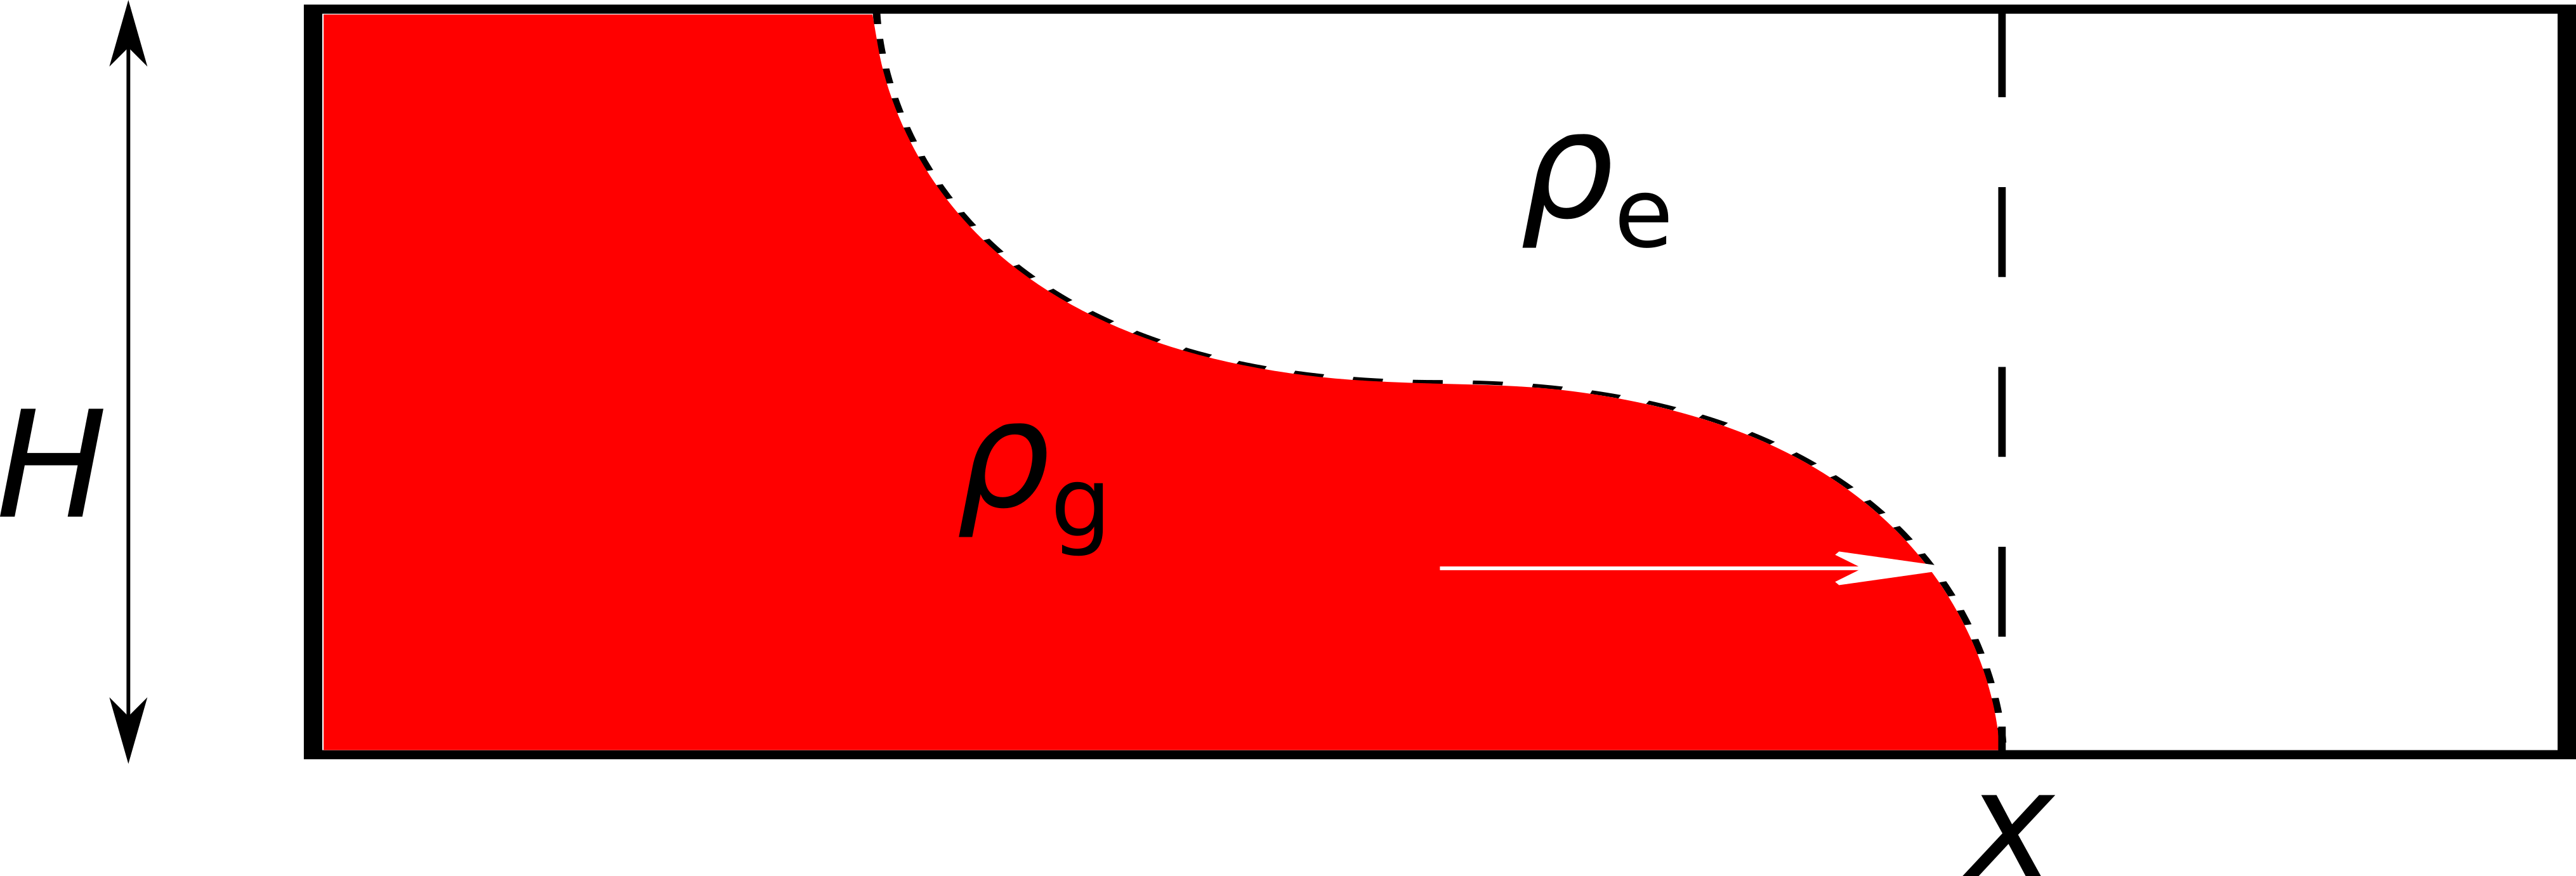
\includegraphics[width=0.75\textwidth]{grav_curr.png}$$
  \caption{Gravity current of density $\rho_{\text{g}}$ propagating in a fluid of depth $H$ and density $\rho_{\text{e}}$. The position of the current head is denoted by $x$. \label{fig:grav_curr}}
\end{figure}

For the current position $x$, we need to scale $x$ by a lengthscale in the problem. In this case, the appropriate choice is the flow depth $H$. Therefore, the dimensionless current head position is $x' = x / H$.

For the time $t$, we need to find some combination of quantities with units of time. This must be constructed from the parameters involved in the problem: $H$, $\rho_{\text{g}}$, $\rho_{\text{e}}$ and $g$. The suitable combination is $(H / g')^{1/2}$ where $g' = (\rho_{\text{g}} - \rho_{\text{e}}) / \rho_{\text{e}}$ is the reduced gravity. Therefore the dimensionless time is $t' = t (g' / H)^{1/2}$.


\end{document}

